\documentclass{article}

\usepackage[final]{neurips_2020}
\usepackage[utf8]{inputenc} % allow utf-8 input
\usepackage[T1]{fontenc}    % use 8-bit T1 fonts
\usepackage{hyperref}       % hyperlinks
\usepackage[pdftex]{graphicx}
\usepackage{url}            % simple URL typesetting
\usepackage{booktabs}       % professional-quality tables
\usepackage{amsfonts}       % blackboard math symbols
\usepackage{nicefrac}       % compact symbols for 1/2, etc.
\usepackage{microtype}      % microtypography

\title{Magneto-optical Kerr effect and magnetic anisotropy}

\author{
Umur Can Kaya\\
5410770\\
\texttt{umurcan.kaya@gmail.com}\\
\And
Rohit Sharma\\
number here\\
\texttt{rohitshep@gmail.com}\\
}

\begin{document}

\maketitle

\begin{abstract}
Abstract here.
\end{abstract}

\section{Introduction}
\clearpage
\section{Experimental setup}
\subsection{Magneto-optical Kerr effect}
The experimental setup is shown in figure \ref{fig:exp_setup}.
\begin{figure}[h!]
\centering
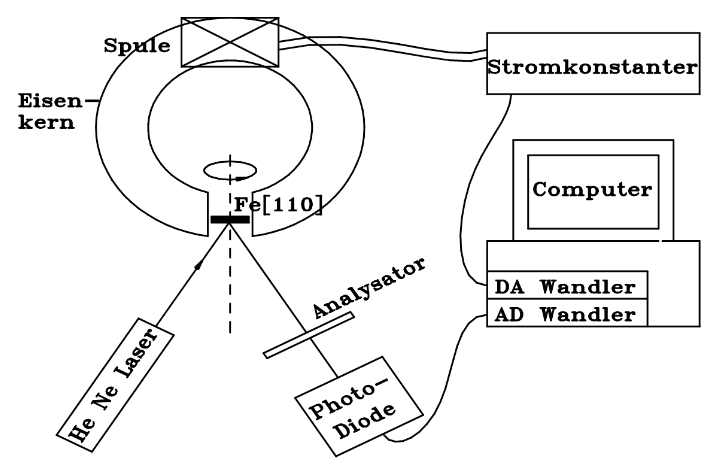
\includegraphics[width=0.6\linewidth]{LAB/MOKE/experimental_setup.PNG}
\caption{Sketch of the experimental setup for MOKE.}
\label{fig:exp_setup}
\end{figure}
\subsection{Kerr microscope}
A Kerr microscope, which utilizes polar MOKE geometry, is used to visualize the magnetic domains of the rare-earth metal. The microscope is equipped with a charge-coupled device (CCD) camera that converts the light reflected from the sample to electronic signal. The external magnetic field which the sample is being subjected to is generated by an electromagnet.
\section{Tasks}
\subsection{Magnetic field calibration}
\subsection{Magnetic anisotropy}
\subsection{Contrast and Kerr rotation}
\subsection{Kerr microscopy}

\section{Discussion}


\section*{References}

[1] Alexander, J.A.\ \& Mozer, M.C.\ (1995) Template-based algorithms for
connectionist rule extraction. In G.\ Tesauro, D.S.\ Touretzky and T.K.\ Leen
(eds.), {\it Advances in Neural Information Processing Systems 7},
pp.\ 609--616. Cambridge, MA: MIT Press.

[2]

\end{document}
